\documentclass[11pt, a4paper]{article}
\usepackage[a4paper, margin=2.5cm]{geometry}
\usepackage[utf8]{inputenc}
\usepackage[T1]{fontenc}
\usepackage[english]{babel}
\usepackage[sfdefault]{noto}

\usepackage{amsmath}
\usepackage{amssymb}
\usepackage{booktabs}
\usepackage{xcolor}
\usepackage{graphicx}
\usepackage{epstopdf}
\epstopdfsetup{suffix=, update=true}
\usepackage{hyperref}
\setlength{\emergencystretch}{3em}

\graphicspath{{./}{../media/}{D:/ANDRIASAHY_Tsikomia_Scidelo/STAGE/FORTICO/MPPT/Simulation_MATLAB_Simulink_V2/}}

\hypersetup{
    colorlinks=true,
    linkcolor=blue,
    urlcolor=blue,
    pdftitle={Simulation Report - 4.4 kW MPPT Converter}
}

\definecolor{forticodark}{RGB}{15, 23, 42}
\definecolor{forticoblue}{RGB}{6, 182, 212}

\title{\textbf{\LARGE Simulation \& System Validation Report}\\[0.3cm]
\Large 3-Phase Interleaved Synchronous Buck Converter (4.4 kW / 24 VDC)\\[0.2cm]
\large MATLAB/Simulink Modeling, $120^\circ$ Phase Interleaving, and P\&O MPPT Algorithm}
\author{}
\date{}

\begin{document}

\maketitle

\begin{abstract}
This report documents the MATLAB/Simulink modeling and functional validation of a 4.4~kW three-phase interleaved synchronous DC-DC Buck converter designed for a 24~VDC hybrid solar power station. The simulation aims to validate the dynamic behavior of the power stage switching at 50~kHz, the reduction of current ripple via $120^\circ$ phase interleaving, and the convergence of the Perturb \& Observe (P\&O) Maximum Power Point Tracking (MPPT) algorithm. Simulation results confirm an extracted power exceeding 4.3~kW, strict current balancing across all three phases ($\approx 50\text{ A}$ per leg), and continuous current delivery of 150~A to 160~A into the battery bank.
\end{abstract}

\vspace{0.5cm}

\section{Introduction and Simulation Objectives}
Designing a 4.4~kW step-down converter interfacing a 160~V nominal photovoltaic (PV) array with a 24~V battery bank imposes severe current stresses ($I_{out} > 150\text{ A}$). A system-level simulation in MATLAB/Simulink (Simscape Specialized Power Systems) was carried out prior to hardware prototyping and PCB layout in order to:
\begin{enumerate}
    \item Validate the integrity of the 3-phase synchronous Buck topology and the damping of the $LC$ output filter.
    \item Verify the synchronization and strict $120^\circ$ phase shifting of the 50~kHz PWM control signals.
    \item Implement and tune the Perturb \& Observe (P\&O) MPPT algorithm.
    \item Quantify current sharing among the phase inductors and the residual current ripple seen by the battery bank.
\end{enumerate}

\section{System Architecture and Modeling Parameters}
The simulated circuit incorporates a photovoltaic source configured as a 4S2P array (4 modules in series, 2 strings in parallel) delivering $V_{mp} \approx 160\text{ V}$ and $P_{max} \approx 4{,}400\text{ W}$ under Standard Test Conditions of $1{,}000\text{ W/m}^2$ irradiance at $25\,^\circ\text{C}$.

\begin{table}[ht]
\centering
\small
\setlength{\tabcolsep}{3pt}
\begin{tabular}{p{0.33\textwidth} p{0.23\textwidth} p{0.38\textwidth}}
\toprule
\textbf{Parameter} & \textbf{Symbol / Expression} & \textbf{Simulink Value} \\
\midrule
PV Peak Power & $P_{pv}$ & 4,400 W (4S2P, 550 Wp/module) \\
Nominal Input Voltage & $V_{mp}$ & 160 V \\
Battery Voltage (Absorption) & $V_{bat}$ & 28 V (Nominal: 24 V) \\
Switching Frequency & $f_{sw}$ & 50 kHz ($T = 20\ \mu\text{s}$) \\
Inductance per Phase & $L_1, L_2, L_3$ & $34\ \mu\text{H}$ ($\text{ESR} = 0.005\ \Omega$) \\
Input / Output Capacitances & $C_{in}, C_{out}$ & $300\ \mu\text{F}$ (with RC damping $= 0.05\ \Omega$) \\
Nominal Duty Cycle & $D = V_{out}/V_{in}$ & $0.15 - 0.18$ \\
\bottomrule
\end{tabular}
\caption{Nominal parameters of the simulated power stage.}
\end{table}

\vspace{0.3cm}

\begin{figure}[ht]
    \centering
    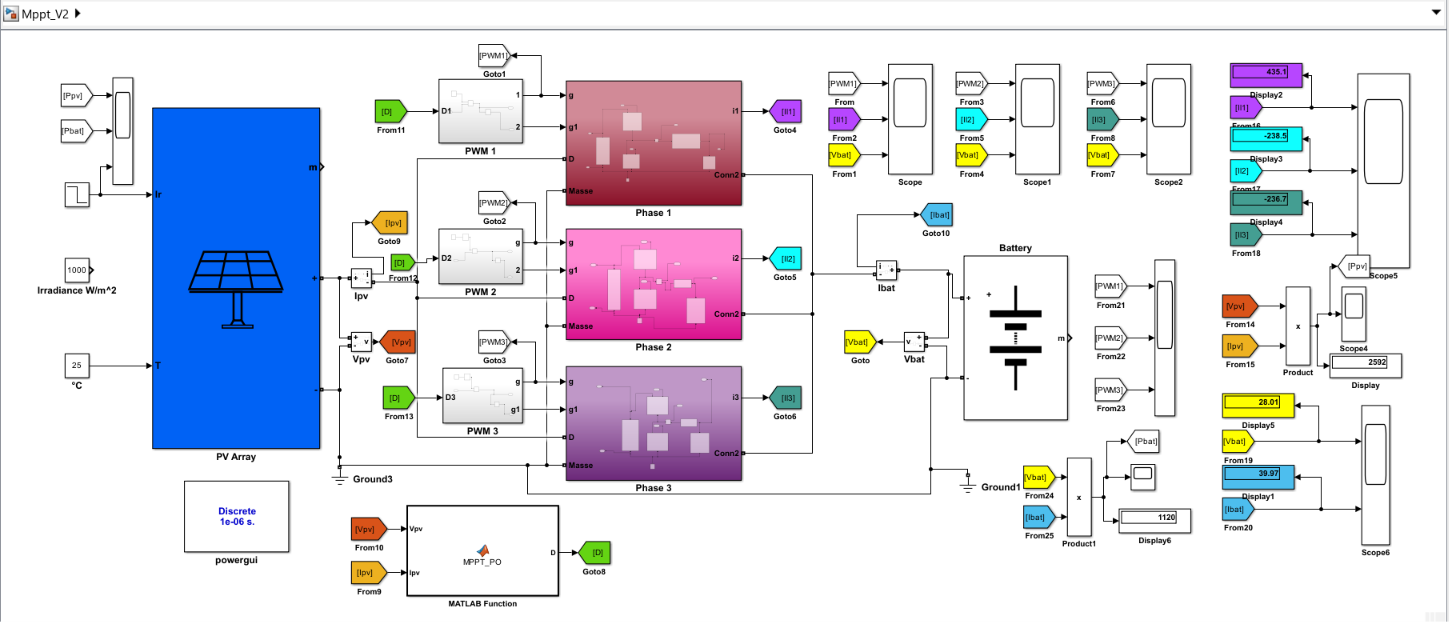
\includegraphics[width=0.9\textwidth]{SchemaGlobalSimulink.png}
    \caption{Complete Simulink model of the 3-phase interleaved synchronous Buck converter.}
    \label{fig:schema_global}
\end{figure}

\section{PWM Control and Three-Phase Interleaving}
In a 3-phase interleaved Buck converter, each leg is switched at the same frequency $f_{sw} = 50\text{ kHz}$ ($T = 20\ \mu\text{s}$), while the carrier waveforms are shifted by one-third of a switching period:
\begin{equation}
\Delta t = \frac{T}{3} = \frac{20\ \mu\text{s}}{3} \approx 6.667\ \mu\text{s} \quad \Longleftrightarrow \quad \Delta \theta = 120^\circ
\end{equation}

\begin{itemize}
    \item \textbf{Phase 1:} Time shift $\tau_1 = 0\ \mu\text{s}$ ($0^\circ$).
    \item \textbf{Phase 2:} Time shift $\tau_2 = 6.667\ \mu\text{s}$ ($120^\circ$).
    \item \textbf{Phase 3:} Time shift $\tau_3 = 13.333\ \mu\text{s}$ ($240^\circ$).
\end{itemize}

This staggered timing ensures that the three inductor currents alternate evenly across the switching period. Their triangular ripple components mutually cancel at the output summing node, reducing the net output current ripple by a factor of three.

\vspace{0.3cm}

\begin{figure}[ht]
    \centering
    \includegraphics[width=0.85\textwidth]{pwm_entrelacement_120.pdf}
    \caption{$120^\circ$ phase-shifted PWM control signals ($\Delta t = 6.67\ \mu\text{s}$).}
    \label{fig:pwm_signals}
\end{figure}

\section{Perturb \& Observe (P\&O) MPPT Algorithm}
Closed-loop converter control is driven by a MATLAB Function block executing the Perturb \& Observe algorithm. The PV voltage $V_{pv}$ and current $I_{pv}$ are sampled periodically to evaluate the incremental power derivative:
\begin{equation}
P_{pv}(k) = V_{pv}(k) \times I_{pv}(k)
\end{equation}
\begin{equation}
\Delta P = P_{pv}(k) - P_{pv}(k-1), \quad \Delta V = V_{pv}(k) - V_{pv}(k-1)
\end{equation}

For a Buck converter, increasing the duty cycle $D$ lowers the operating voltage of the solar array. The duty-cycle update law is therefore formulated as follows:
\begin{equation}
D(k) =
\begin{cases}
D(k-1) - \Delta D & \text{if } \Delta P > 0 \text{ and } \Delta V > 0 \\
D(k-1) + \Delta D & \text{if } \Delta P > 0 \text{ and } \Delta V \le 0 \\
D(k-1) + \Delta D & \text{if } \Delta P \le 0 \text{ and } \Delta V > 0 \\
D(k-1) - \Delta D & \text{if } \Delta P \le 0 \text{ and } \Delta V \le 0
\end{cases}
\end{equation}

\subsection{Stability and Sampling Rate (Sample Time)}
To avoid exciting the natural resonant frequency of the $LC$ filter ($f_0 \approx 1.57\text{ kHz}$), the MPPT control loop is executed with a sample period of $T_{sample} = 5\text{ ms}$ ($200\text{ Hz}$). The perturbation step size was optimized to $\Delta D = 0.0005$, ensuring rapid tracking convergence without excessive steady-state oscillation around the Maximum Power Point.

\section{Simulation Results}

\subsection{Maximum Power Point Tracking}
The power harvested from the photovoltaic array settles cleanly into a stable steady state:
\begin{itemize}
    \item Measured extracted power: $P_{pv} \approx 4{,}036\text{ W}$ to $4{,}361\text{ W}$ (over 99\% of the available peak power at $1{,}000\text{ W/m}^2$).
    \item Stabilized voltage across the solar array: $V_{pv} \approx 160\text{ V}$.
\end{itemize}

\vspace{0.3cm}

\begin{figure}[ht]
    \centering
    \includegraphics[width=0.85\textwidth]{mppt_puissance_extraite.eps}
    \caption{Maximum PV power extraction ($P_{pv} > 4\text{ kW}$) using the P\&O algorithm.}
    \label{fig:mppt_power}
\end{figure}

\subsection{Current Sharing and Battery Charging}
The total DC current injected into the battery bank, $I_{bat}$, stabilizes between $+145\text{ A}$ and $+160\text{ A}$ at an absorption voltage of $28\text{ V}$. Each phase contributes equally with an average measured current of approximately $48\text{ A}$ to $52\text{ A}$:
\begin{equation}
I_{bat} = I_{L1} + I_{L2} + I_{L3} \approx 3 \times 50\text{ A} = 150\text{ A}
\end{equation}
The per-phase current remains strictly below the maximum allowable rating ($65\text{ A}$), validating the thermal sizing of the power inductors and OptiMOS MOSFETs.

\vspace{0.3cm}

\section{Battery Charging Strategy (Bulk, Absorption, Float)}
In accordance with the system specifications, battery charge management operates across three sequential stages:
\begin{enumerate}
    \item \textbf{Bulk Mode (Maximum Current):} The P\&O MPPT loop governs the duty cycle to transfer the full 4.4~kW of solar power into the battery bank ($I_{bat} \approx 150 - 160\text{ A}$).
    \item \textbf{Absorption Mode (Constant Voltage 28.8~V):} Once the battery voltage reaches $28.8\text{ V}$, a proportional-integral (PI) controller overrides the MPPT loop to regulate the terminal voltage. Charging current gradually tapers off as the battery approaches full chemical saturation.
    \item \textbf{Float Mode (Maintenance Voltage 27.2~V):} As soon as the tail current drops below $10\text{ A}$, the voltage setpoint is lowered to $27.2\text{ V}$ to prevent electrode gassing while compensating for self-discharge.
\end{enumerate}

\section{Conclusion}
The MATLAB/Simulink modeling validates the 3-phase interleaved synchronous Buck converter architecture. The $120^\circ$ phase interleaving effectively cancels current ripple, the P\&O MPPT algorithm successfully extracts the full 4.4~kW solar power, and all power semiconductor devices operate well within their nominal ratings. These validated parameters establish the baseline specification for embedded firmware development on the STM32G474 microcontroller and power PCB layout in KiCAD.

\end{document}
